\documentclass[11pt, oneside, fleqn]{article}
\usepackage[top=1.25in, bottom=1.25in]{geometry}
\geometry{letterpaper}
\usepackage[parfill]{parskip}			% Activate to begin paragraphs with an empty line rather than an indent

\usepackage{amssymb}
\usepackage{amsmath}
\usepackage{graphicx}
\usepackage{hyperref}

\pagestyle{empty}	% No page number in the footer.
\begin{document}
  \begin{center}
  \LARGE{Exploring Carl de Marcken's Word Segmentation}\\[0.5em]
  \large{Brian Hempel and Yuxi Chen}\\[0.5em]
  \large{June 8, 2016}\\[0.5em]
  \end{center}

  \vspace{1em}

  \section{Introduction}

  Carl de Marcken, in his PhD thesis ``Unsupervised Language Acquisition'', attempted to learn words given a large corpus of sentences devoid of all spaces and punctuation, similar to how children learn words from no prior information. In his thesis, de Markcen models learning by searching for a lexicon that minimizes the combined description length of the input and the lexicon together. Both words in the lexicon and sentences are represented by composing smaller words. His method iteratively adds and deletes new lexicon entries based on the goal. The hope is that patterns in the final lexicon reflect the underlying mechanisms and parameters of the language that generated the input.
  
  \section{What We Did}

  We focus on re-implementing the learning algorithm of Carl de Marcken's PhD thesis. The general idea is to start with the simplest lexicon, then iteratively refine the entries of the lexicon to reduce the description length until convergence. 
  
  In the first part of each iteration, stochastic properties are optimized assuming a fixed lexicon. The expectation-maximization algorithm is used to approach a locally optimal set of probabilities for each word in the lexicon.
 
  After optimizing the stochastic properties, the algorithm adds words to the lexicon. Candidate words are composed of pairs of existing words that occur together at least twice in the soft counts calculated over the lexicon and the corpus. An estimation is made of the change in description length presuming the word is added to the lexicon and its parts possibly deleted. If the description length will decrease, the pair is to the lexicon.

  After another bout of stochastic optimization, a similar estimation is used to delete words from the lexicon. 
  
  We run the algorithm for 15 iterations. De Marcken discussed convergence criteria in his thesis, but chose to simply run his algorithm for 15 iterations for simplicity and to avoid the algorithm entering a loop where the same words are added and deleted repeatedly on successive iterations due to inaccuracy in the estimates used to predict changes in the description length.
  
  \subsection{Implementation Notes}
  
  For the forward-backward stochastic optimization step, we calculate probabilities using log probabilities to avoid floating point underflow.

  On the input corpus, we downcase the input and delete all non-alphanumeric characters, including whitespace. In order to speed up processing, we use PyPy instead of CPython. With PyPy and several internal optimizations, a full run on the entire Brown Corpus takes roughly five hours.
  
  Our implementation is available at \href{https://github.com/brianhempel/demarcken_word_segmentation}{https://github.com/brianhempel/demarcken\_word\_segmentation}.
  
  Our tool produces several output files:

  \begin{itemize}
    \item The found lexicon, as flat words (one word per line, most common word first).
    \item The true lexicon, as flat words (one word per line, most common word first).
    \item The found segmentation of the corpus, as flat words.
    \item The found segmentation of the corpus, with words given by their full nested representation.
    \item The true segmentation of the corpus, as flat words. 
  \end{itemize}

	We consider hyphens and whitespace as true word separators in the original corpus. A glance at the Brown corpus suggested to us that most hyphenated utterances should be considered multiple words.

  \subsection{Evaluation Criteria}

	In the algorithm, lexicon entries are composed of a hierarchy of other lexicon entries. To judge performance, de Marcken compared these hierarchies with the true segmentation. De Marcken's recall rate is the proportion of the words in the true segmentation that also appear at some level of the algorithm's hierarchical parse of the input. The crossing-brackets rate (somewhat analogous to precision) measures a concept called crossing-bracket violations. A word in the true segmentation is considered a crossing bracket violation if a word in any level of the found hierarchical representation starts/ends in the middle of the true word but also crosses over into a neighboring word.
    
    With these metrics, de Marcken claims a recall of 90.5\% and a crossing-brackets rate of 1.7\%, which makes his work sound highly performant.

	The problem is that we don't know which level in the hierarchy has the correct word. For our evaluation, we consider only the top level of hierarchy as the found word for segmentation.

	We measure the performance of the algorithm and our experiments below by calculating the precision and recall for three different comparisons against the true segmentation:
	
	\begin{enumerate}
		\item We compare the set of word break locations found in the corpus to the the true word break locations.
		\item We compare the words in the found segmentation to the true words at each corpus location.
		\item We compare the set of words in the found lexicon to the set of words in the true lexicon.
	\end{enumerate}

  \section{Experiments}
  
  We made several different modifications to the baseline algorithm to see how each changes segmentation performance. All tests were performed on the Brown Corpus, which contains 44,195 unique words across 14,342 sentences.

	The various experimental modifications are described below.

  \subsection{Flat Words in Lexicon}
  
  De Marcken uses a nested representation for all words in the lexicon; that is, words are composed of other words. We tend not to think of words as being made up of smaller words, so what if we instead require all words in the lexicon to be represented by sequences of single characters?

  \subsection{Flat Words in Lexicon, Separate Lexicon Probability Model}

	De Marcken's baseline algorithm uses the same probability model for representing words in the lexicon and representing sentences. This method breaks down in the naive ``Flat Words in Lexicon'' model above. Single characters are overrepresented for parsing the corpus, and full words are overrepresented for parsing the lexicon.
	
	Instead, in this experiment we keep a character probability model specifically for representing the words in our lexicon. The word probabilities for the corpus are kept separately.

  \subsection{Flat Words in Lexicon, O(1) Lexicon Probability Model}

	Life experience suggests to us that real words have structure. The zero-order probability model of the previous experiment cannot capture structure. In this experiment we use a first order probability model for representing the words in our lexicon: the probability for each character is conditioned based on the prior character. Thus, character pairs uncommon to words are penalized.
	
	\textit{An implementation detail:} When character pairs probabilities are recalculated, we can't let any probability be 0; otherwise we won't be able to use that character. To avoid this, when counting characters, instead of counting from 0 each character count is instead initialized to the 0-order probability of the character (a number between 0 and 1) and counts are added on top of that.

	\subsection{Variations in Lexicon Entry Cost}
	
	We variously bias the algorithm against word creation by assigning an extra storage cost to words. We tested the algorithm where entries in the lexicon are considered to cost -8/+1/+2/+4/+16/+32/+64 extra bits.

	\subsection{Variations in Minimum Occurrences Required to be a Word}
	
	The baseline algorithm will only consider a word pair as a candidate to be added to the lexicon if the word pair occurs at least twice. We tested raising this requirement to 3, 4, or 5 minimum occurrences before consideration.
 
 \pagebreak
 
   \section{Results}
   
   On the Brown Corpus, de Marcken reports a final lexicon size of 26,026 words and a description length equivalent to 2.33 bits per character. We produce a lexicon of 26,171 words at 2.23 bits per character. Our higher measured compression rate is probably due to minor discrepancies between our implementation and his. Part of de Marcken's thesis discusses a Huffman coding scheme. His paper is unclear, but he may be assuming such a scheme for his compression calculation. We presume an arithmetic coding scheme, which is more efficient.
   
   As shown in the graph of lexicon size below, after about 15 iterations, our algorithm converges.

	\vspace{1em}
  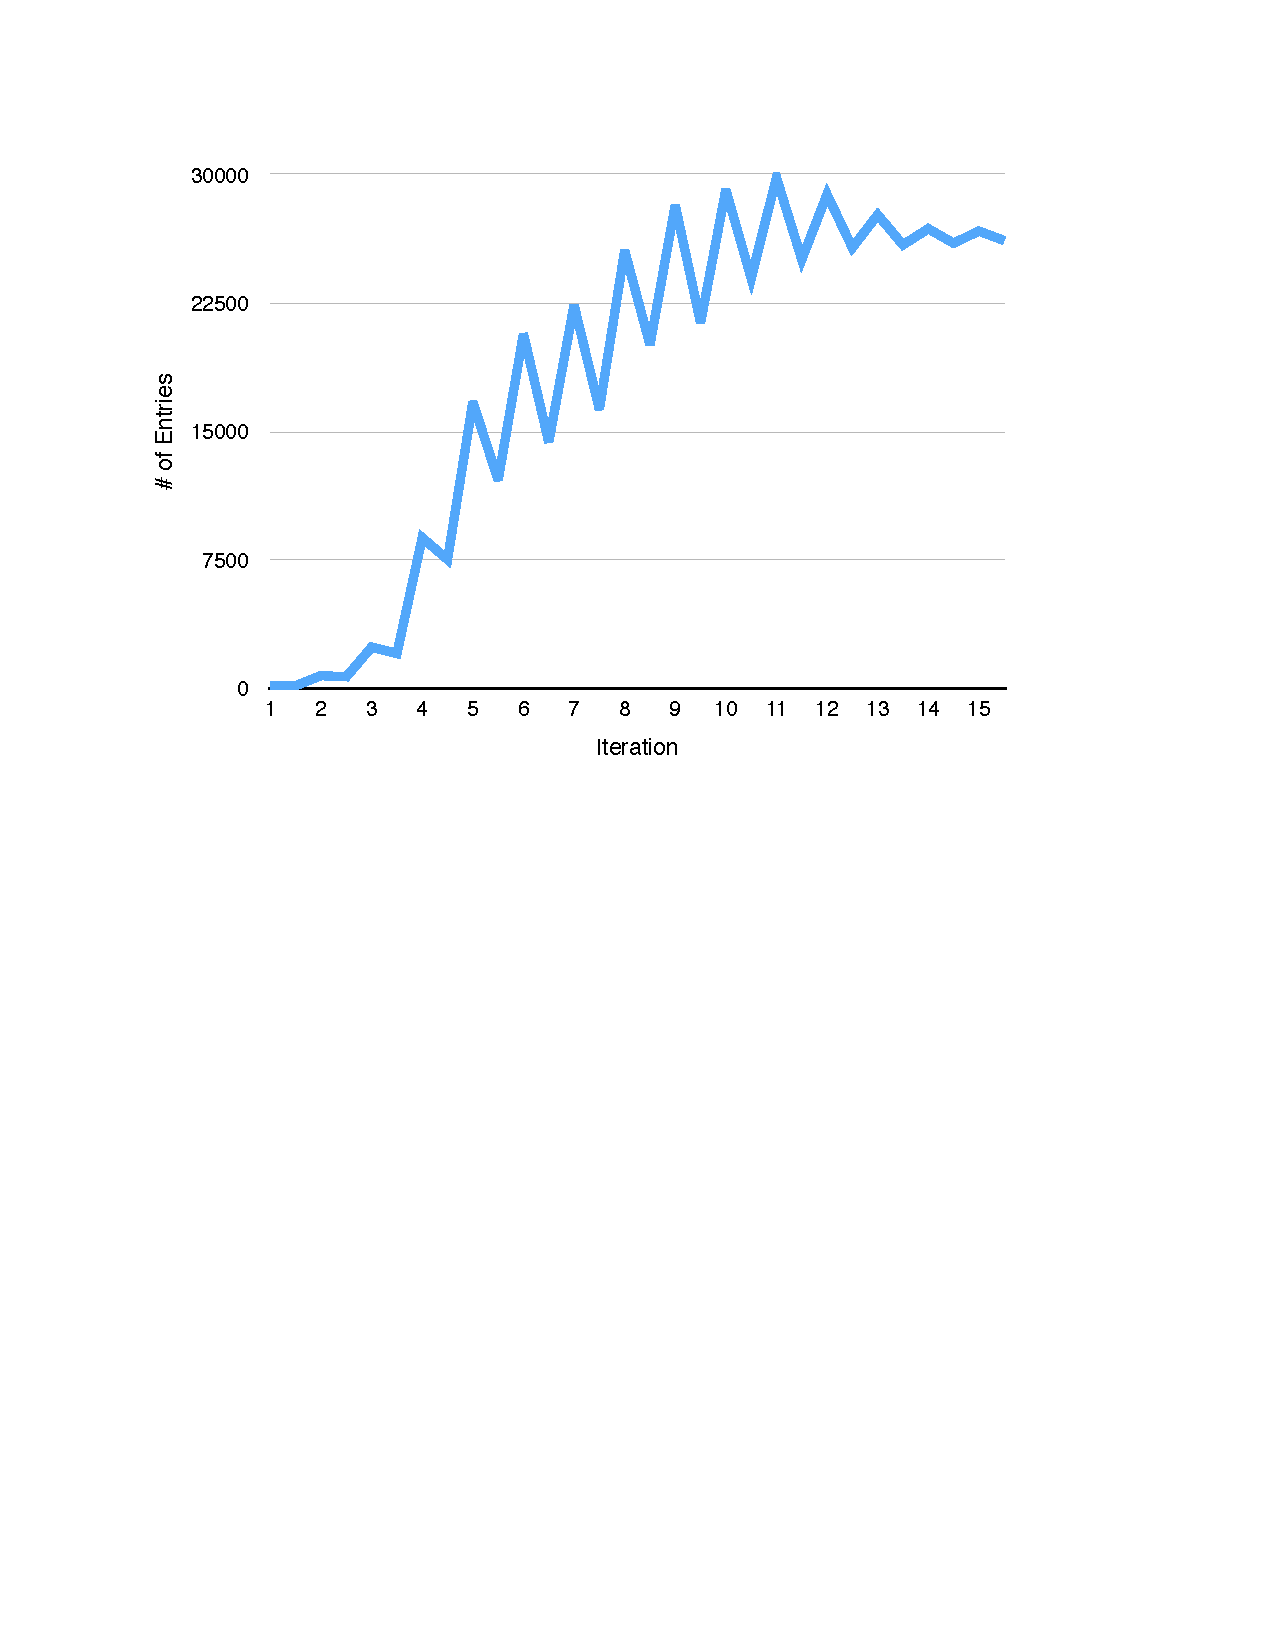
\includegraphics[scale=1.0]{./figure/lexicon_size_per_iteration}

	\pagebreak

  Also, below we plot the relationship between bits per character and iterations. Bits per character decrease iteration by iteration until convergence at about the same time the lexicon stops increasing in size.

  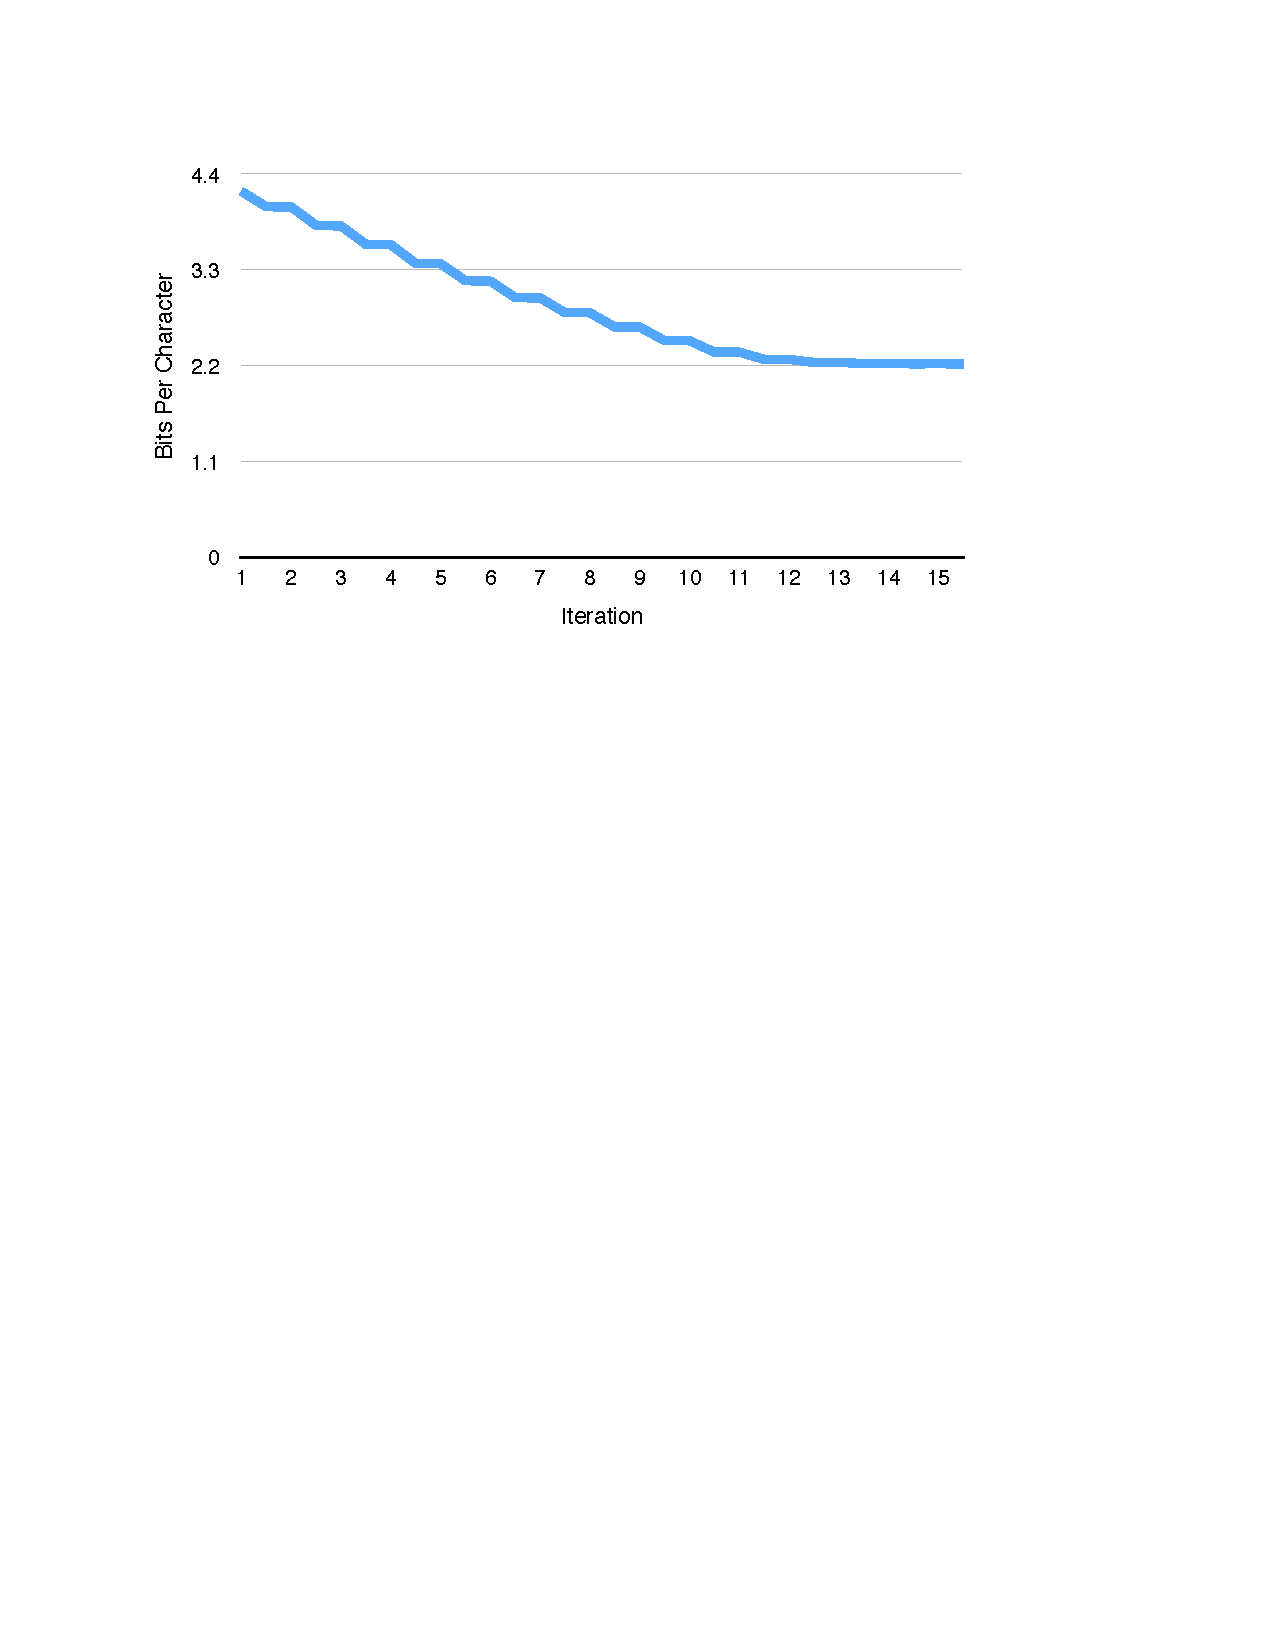
\includegraphics{./figure/bit_of_char_per_iteration.pdf}

  \subsection{Kinds of Errors}

	Of the words in the found segmentation of the corpus, 60\% of the found word locations are exactly correct and 40\% are incorrect in some way. We investigate these incorrect found words and try to categorize what kind of error is being made in each case. As you can see below, about 43\% of these incorrect found words combine two true words together as one found word. 18\% of the found words are a suffix of the of correct word at that location; similarly, 18\% are a prefix of the correct word at the location. 8.7\% of the found words are actually three real words combined together as one word, while 1.6\% comes from the combination of four of more words. We also notice that 6.2\% of the found words are actually a small fragment from the middle of the true word. 3.3\% of the time our tool will find a true word but combine it with a suffix or prefix of its neighbor. The remaining 1.2\% of incorrectly found words come from various other errors, such as the fusion of two words plus a neighboring prefix, or a suffix-prefix fusion across a word boundary.

  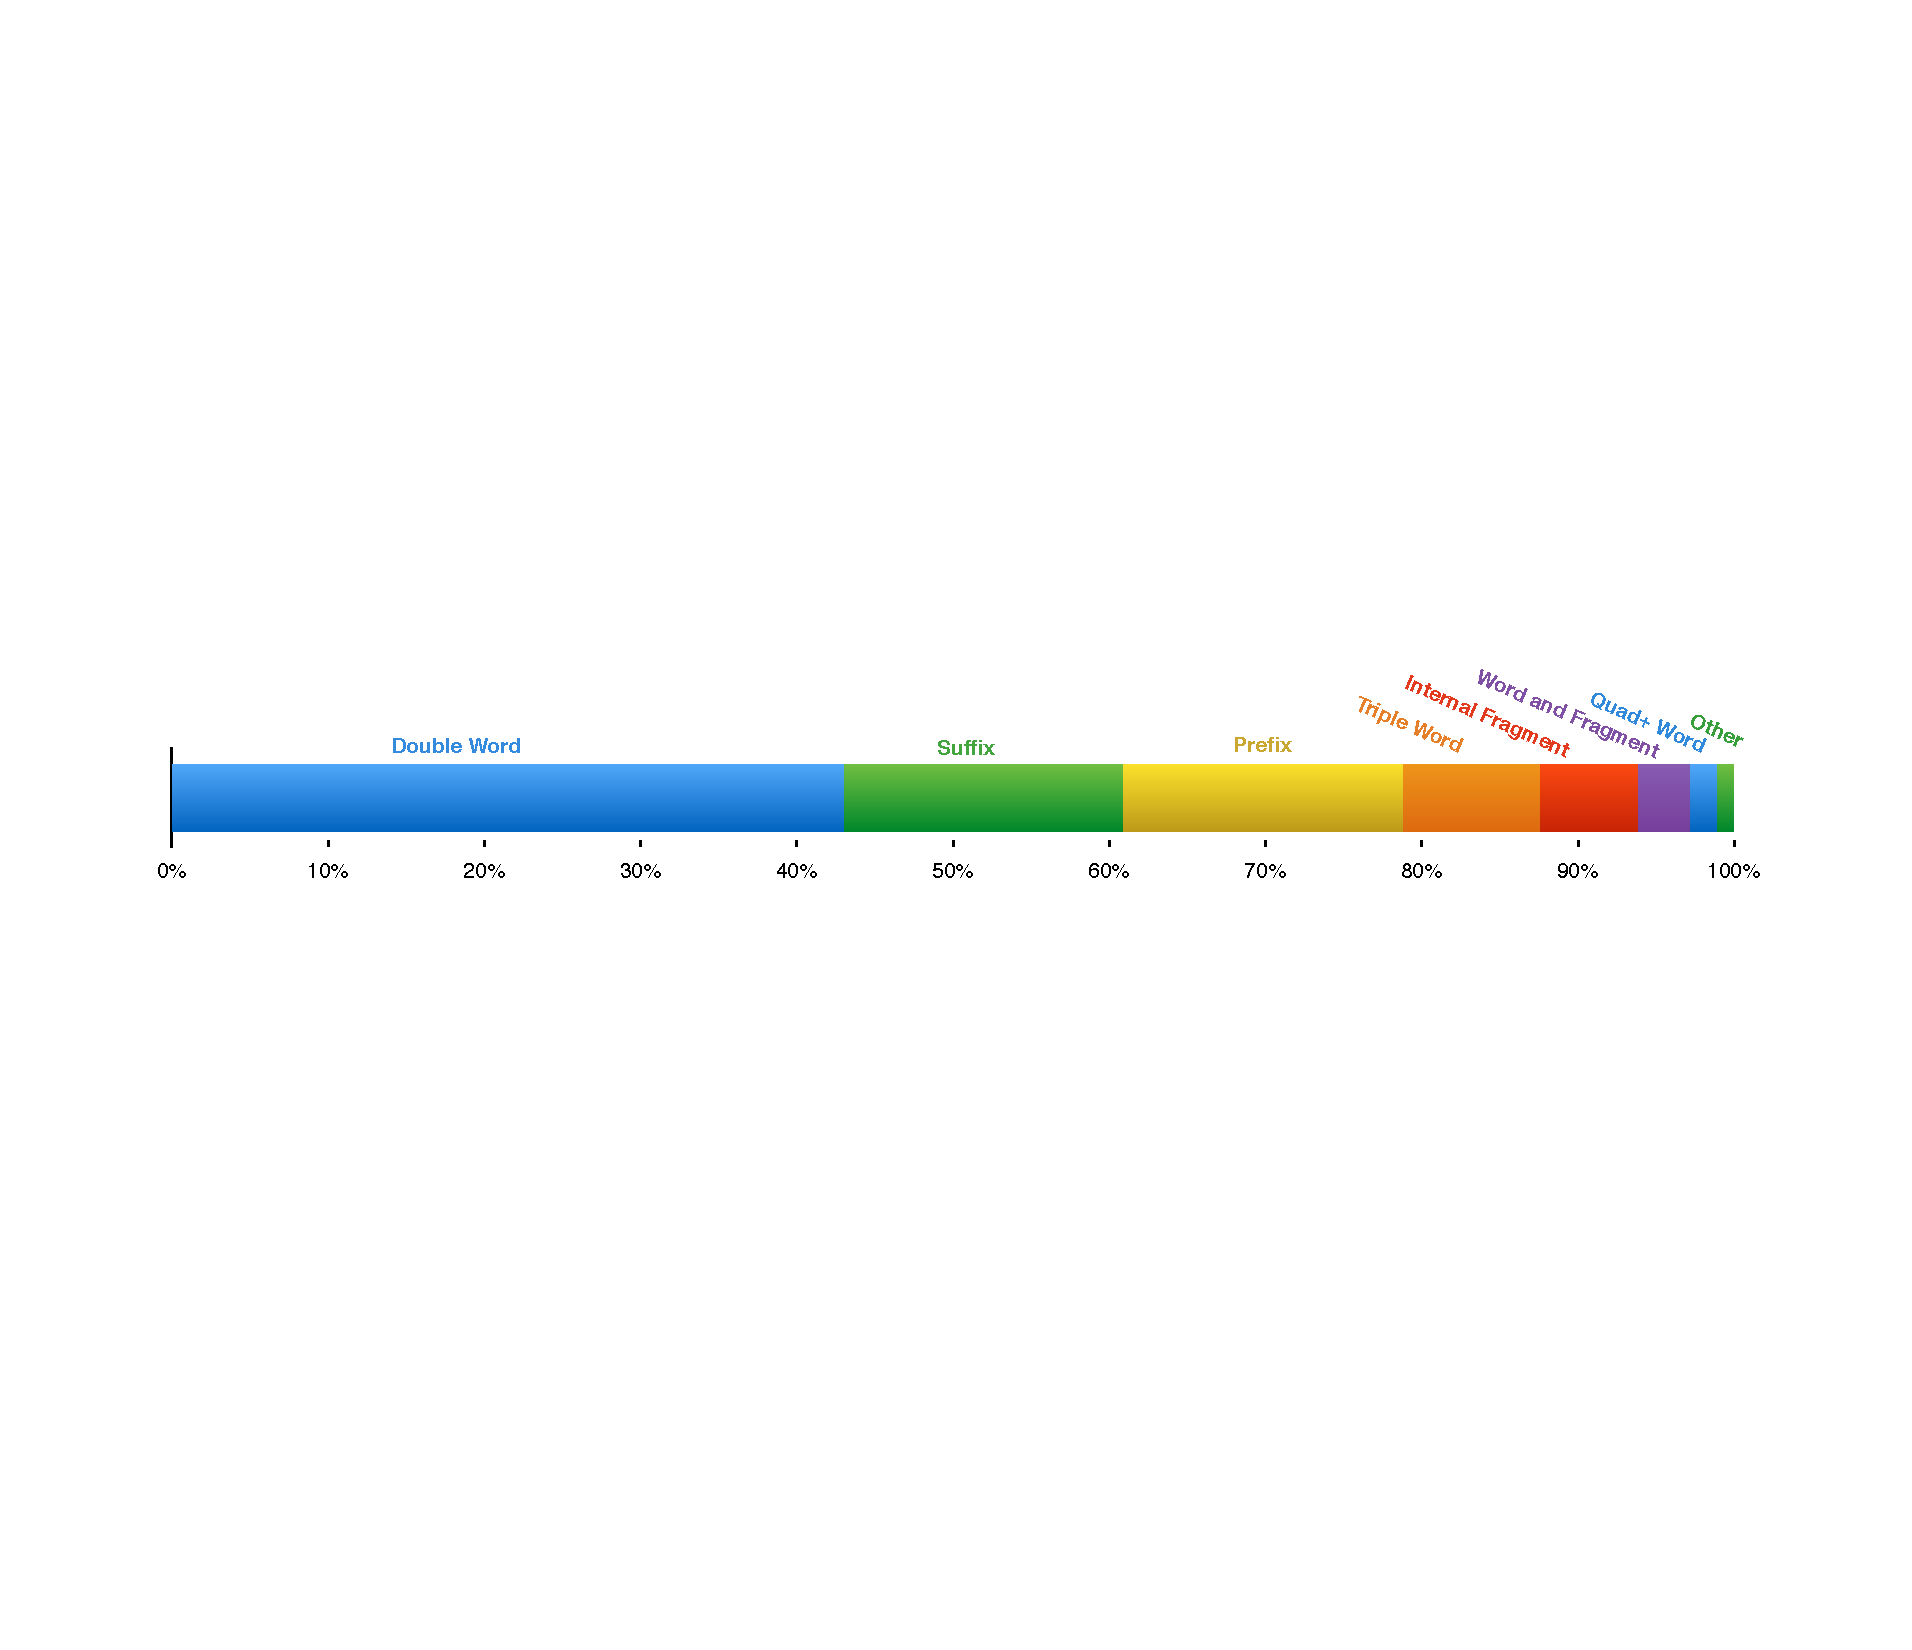
\includegraphics[scale=0.55]{./figure/error_nature_classfier.pdf}

  \subsection{Results for Different Measures of Precision/Recall}
  
  The precision of the set of found corpus word break locations is 87.6\%, while the recall is 74.2\%. This recall value is lower than De Marcken's 90.5\% recall because when calculating recall we only focus on the top level of the hierarchy instead of the whole hierarchy.

  The precision of word locations in the found segmentation is 59.7\%, while the recall is 54.7\%. As we saw from the error kinds section above, lots of our errors come from our tool combining two or more words into a single word, and each such fusion therefore misses two or more word locations. As a result, this recall metric is much lower than De Marcken's. The precision/recall of this metric are also considerably lower than the precision/recall of the break locations metric above, because here there is no partial credit. For a found word location to be correct, its left break must be correct \textit{and} its right break must be correct \textit{and} it must not have spurious breaks in the middle.
  
  When we make our metric the set of words in the found lexicon versus the set of words in the true lexicon, the precision is 52\%, with 30.8\% recall. The low recall is because lots of words occur only once in the Brown Corpus but the algorithm only considers creating a word when a pair occurs more than once. Thus we miss many words. Of the 44,195 unique words in the Brown Corpus, only 26,775 of them occur at least twice. If we consider only these words that occur at least twice, the recall is 50.8\%, which is still not great.

	\pagebreak

  \subsection{Experimental Results}
  
  Note that of the precision/recall graphs below have been focused on the area of interest---none of the axis begin at 0.
  
  \subsection{Effect on Finding Word Breaks in Corpus}

	\vspace{1em}
  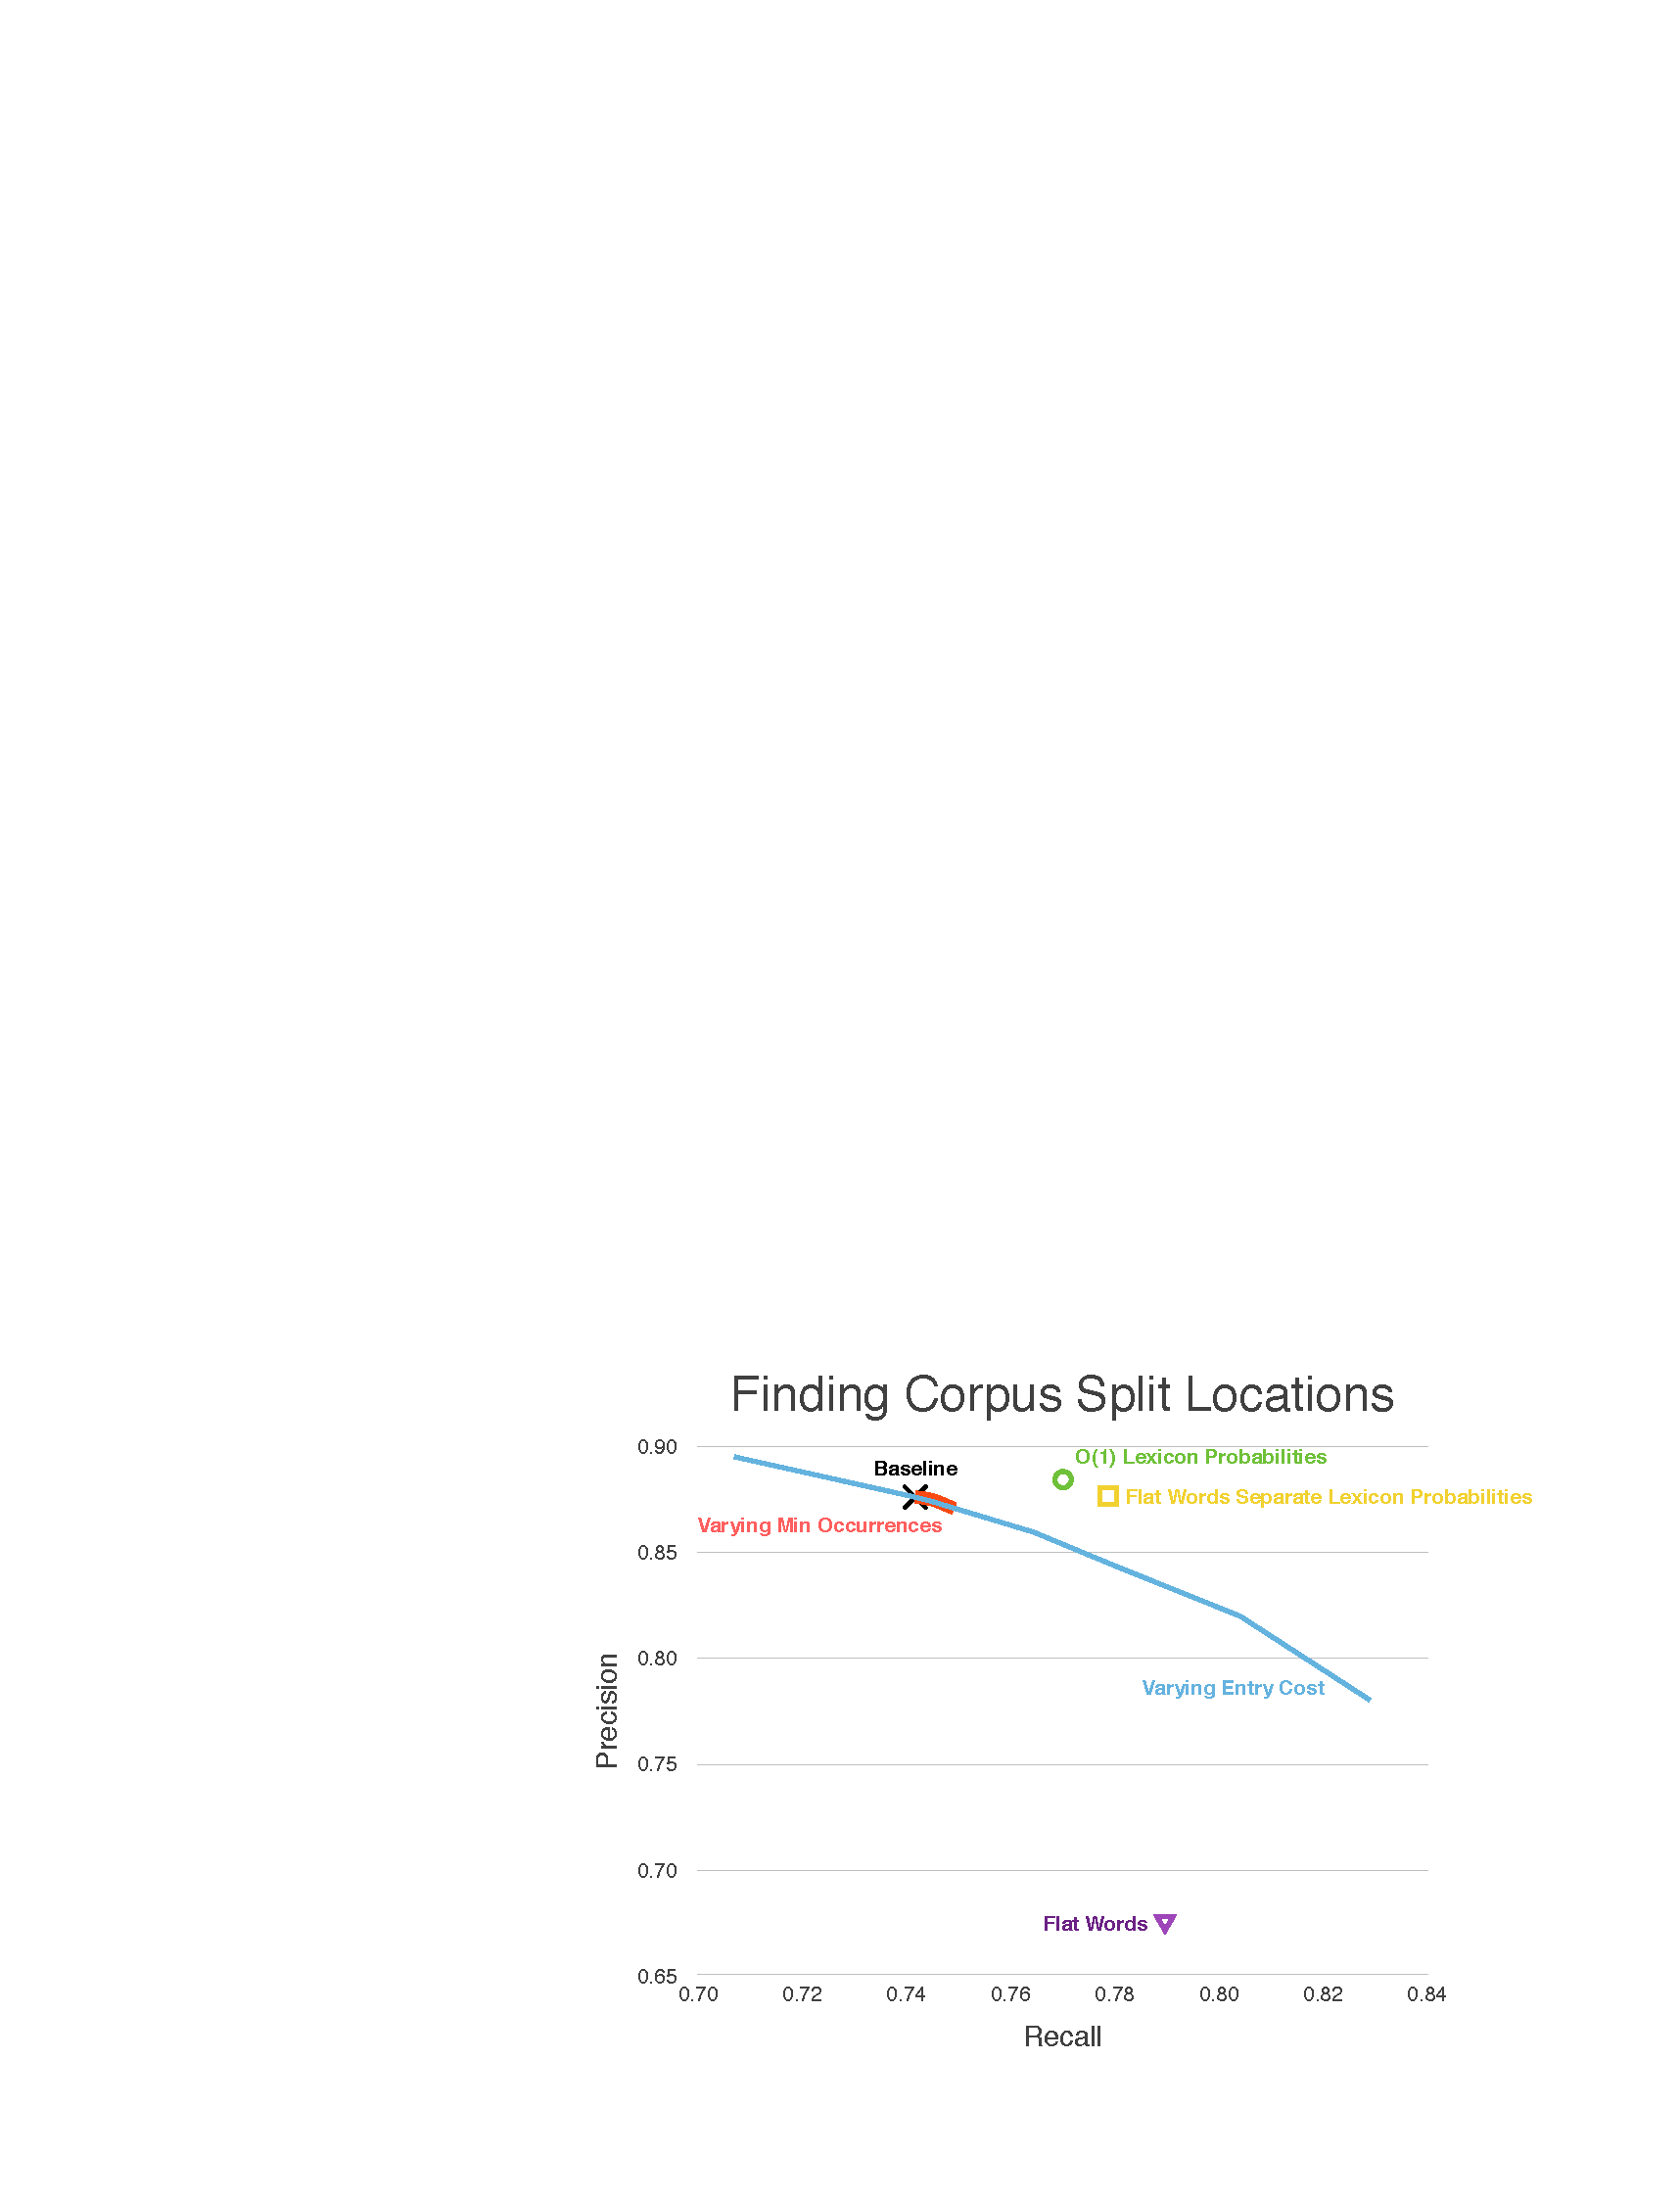
\includegraphics[scale=0.9]{./figure/finding_corpus_split_location.pdf}
  
  Both methods of decreasing lexicon size---requiring words to occur more often before being considered for addition, and imposing extra description length cost for each lexicon entry---increase split position recall in the corpus. Less words means we must use smaller words which means more word breaks.
 
 	Curiously, requiring a word to occur 5 times before it is considered for addition has very little effect on precision or recall (87.1\%/74.9\% precision/recall vs. baseline 87.6\%/74.2\%).

	When lexicon words are represented only by single characters (``Flat Words''), performance is quite poor. The probability of single characters is inflated when parsing the corpus, so in the corpus many parts of sentences are parsed as strings of single-letter words. This creates a lot of word breaks, which raises recall above baseline, but it also creates a lot of word breaks inside true words, lowering precision dramatically (67.5\%/79.0\% precision/recall vs. baseline 87.6\%/74.2\%).

	Simply using a separate character probability table for the lexicon (``Flat Words Separate Lexicon Probabilities'') raises the recall moderately with no effect on precision (87.7\%/77.9\% precision/recall vs. baseline 87.6\%/74.2\%). As seen on the graph, this model performs notably better than the extra cost per entry model.

	The O(1) probability model for the lexicon also performs better than baseline (88.4\%/77.0\% precision/recall vs. baseline 87.6\%/74.2\%) but on this metric it's a toss-up as to whether the O(1) model performs better than the O(0) model above.

  \subsection{Effect on Finding Word Locations in Corpus}

  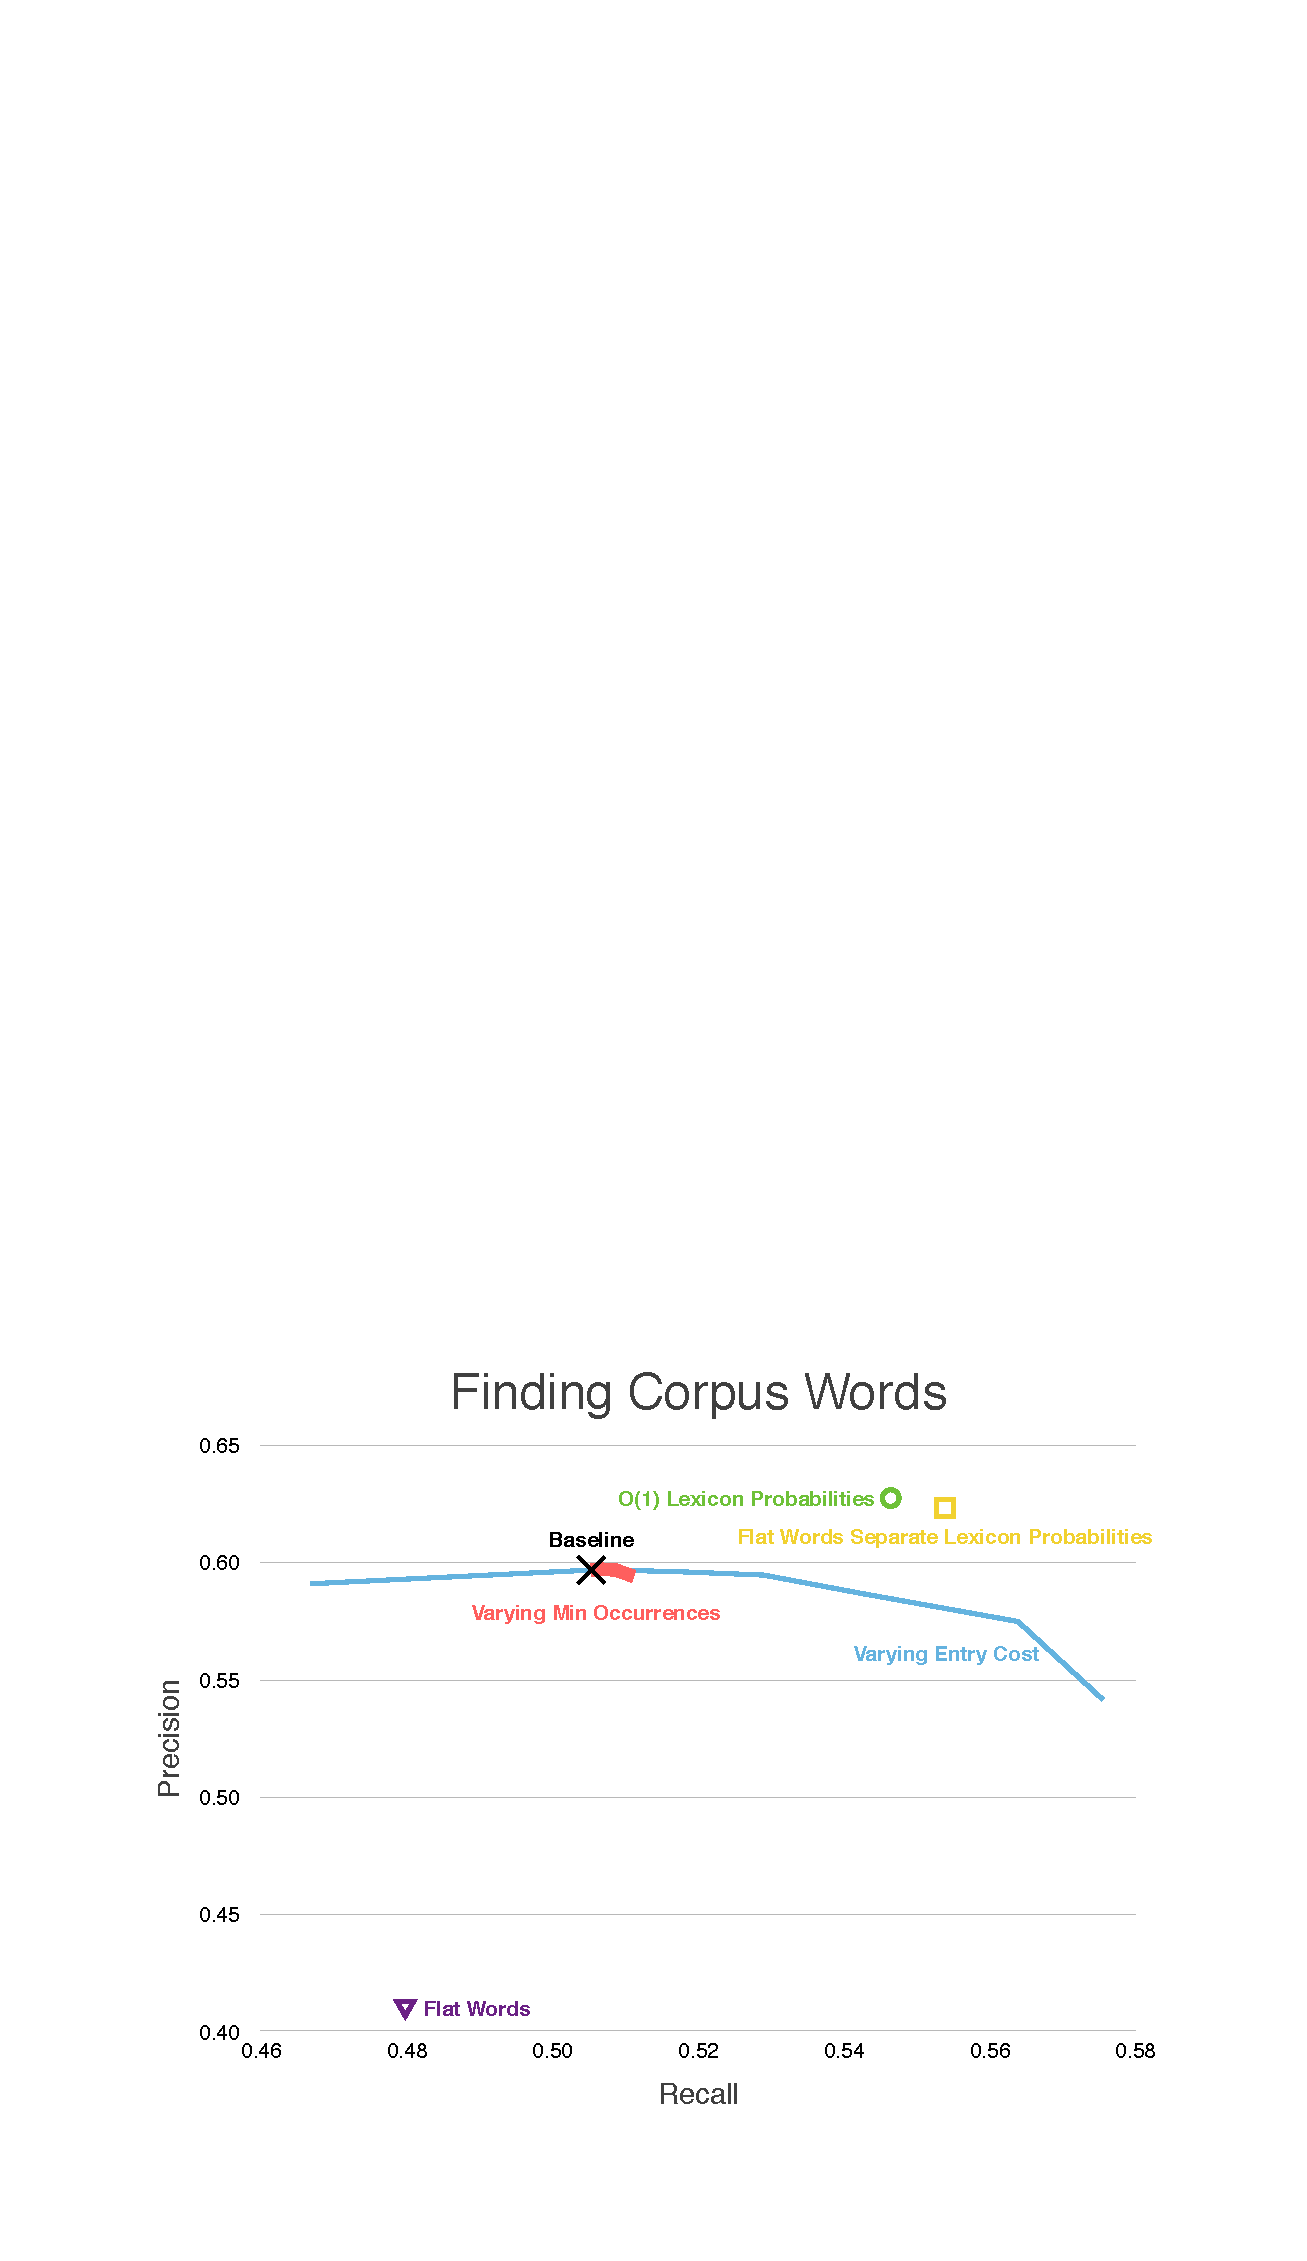
\includegraphics[scale=0.9]{./figure/finding_corpus_word.pdf}
 
    As with the prior metric, requiring a word pair to occur more often before its addition to the lexicon has little effect compared to baseline.

	Above we noted that many of our found words are actual double words fused together. Consequently, raising the cost of a lexicon entry splits up these words, leading to an increase in recall with negligible loss in precision. Not until high lexicon entry cost forces words to split into word parts does precision suffer.

	Since so many of the word location found by the naive ``Flat Words'' model are a-single-letter long, its precision and recall is poor.

	On this metric, both the O(0) (62.3\%/55.4\% precision/recall) and O(1) (62.8\%/54.6\%) lexicon models perform better than baseline (59.7\%/50.5\%), but one is not necessarily better than the other.

	As emphasized above by the precision/recall line for the ``Varying Entry Cost'' experiment, this metric behaves different from standard precision/recall metrics. Usually, high precision requires low recall, and vis versa. However, to get the word correct in every location---that is, 100\% precision---also means that every correct word location is found---100\% recall. For this reason we suggest that, for the word segmentation task, simply the \textit{precision} of found word locations is a sufficient metric by itself, avoiding the subjective tradeoff inherent in precision/recall judgements.
	
	By this metric, the O(1) model performs the best, with 62.8\% of the word locations it finds being correct.

  \subsection{Effect on Finding Lexicon}

  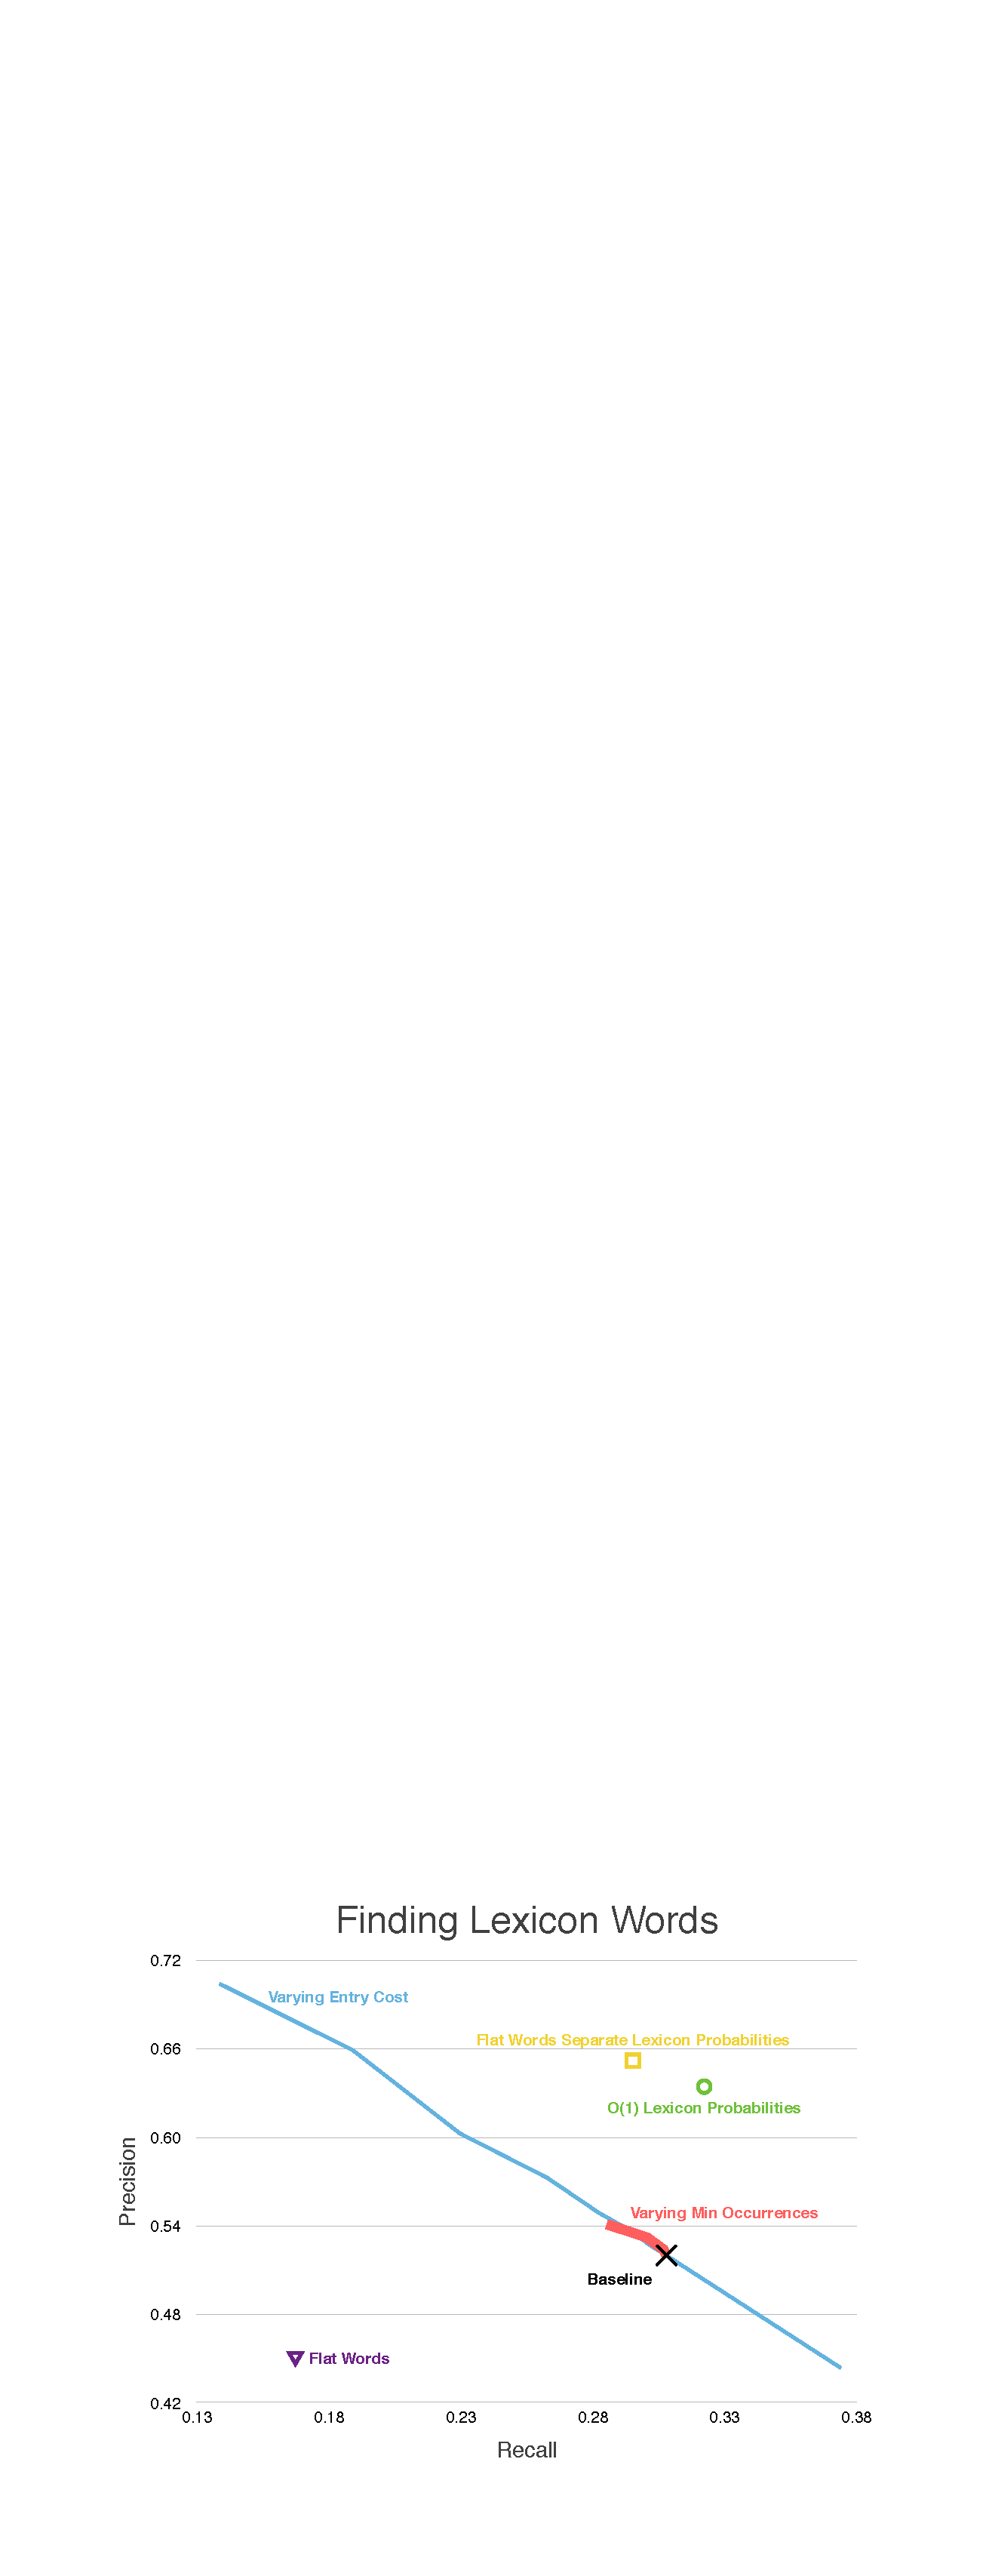
\includegraphics[scale=0.85]{./figure/finding_lexiocn_words.pdf}

	The precision/recall model behavior for words found in the lexicon is flipped compared to the the corpus word break metric. Fewer words in the dictionary created higher word break recall, here fewer words means lower lexicon word recall.

	As before, requiring a word pair to occur more often before its addition to the lexicon has only a little effect compared to baseline.

	Increasing the cost of lexicon entries is quite effective at increasing precision over baseline (70.4\% vs 52.0\%), though it does so by cutting recall in half.

	The naive ``Flat Words'' model performs poorly. Since it represents so many words in the corpus by spelling them out letter by letter, it doesn't form bigger words.

	Interestingly, the O(0) model finds fewer true words than baseline (29.5\% vs 30.8\% recall). It does, however, achieve a significant increase in precision (65.2\% vs 52.0\%).

	The O(1) model performs unequivocally better than baseline, with increased precision and recall (63.4\%/32.2\% vs 52.0\%/30.8\%), but its performance relative to the O(0) model cannot be clearly established.

	\pagebreak

	For curiosity's sake, the final number of entries in the lexicon for each experiment is plotted below. There are few surprises here.

  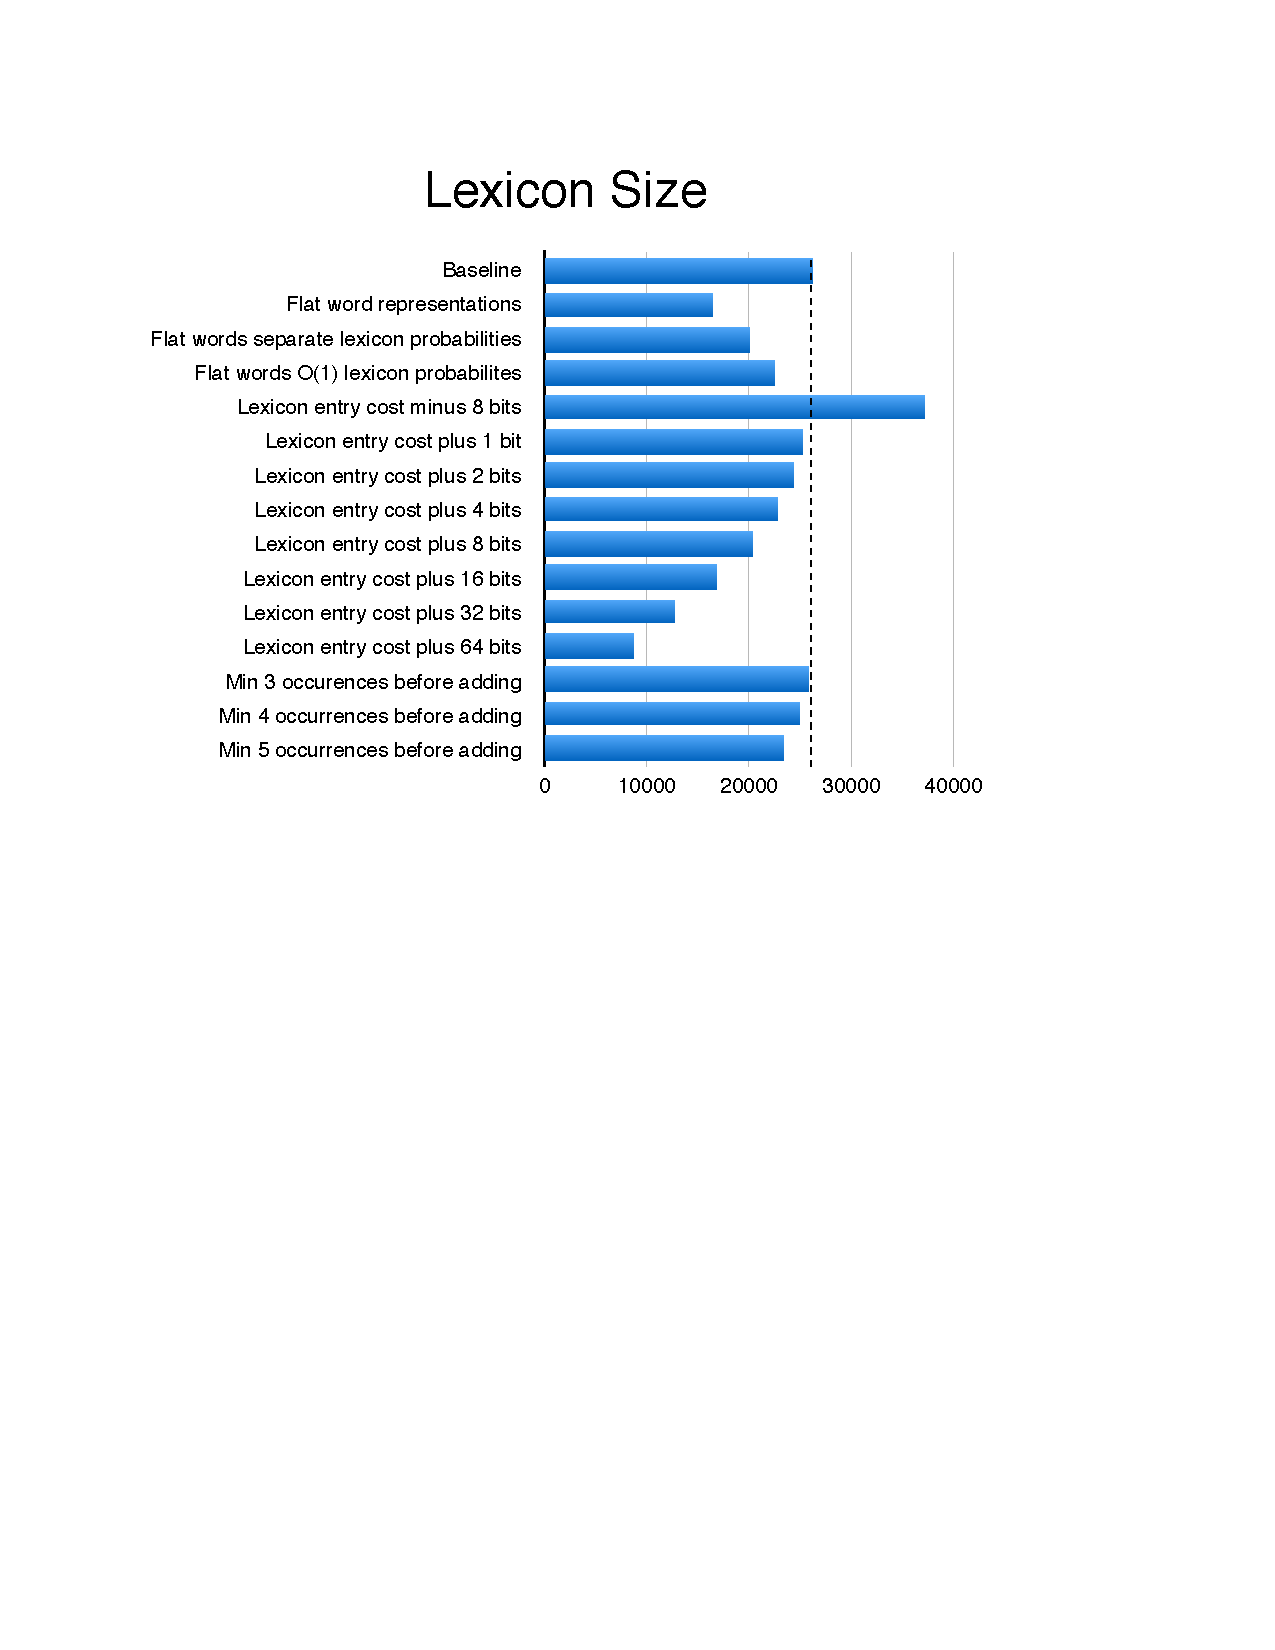
\includegraphics{./figure/lexicon_size.pdf}

  \section{Ideas for Improvement}

  Using a separate probability model to represent the words in the lexicon produced improved performance. In English, only a few words are composed of other words, so using a different representation for the lexicon and the corpus makes sense.
  
  Perhaps this idea can be extended further with explicit negative feedback. Inside this proposal: we partitioned the lexicon entries into two sets: ``word parts'' and ``full words''. Additionally, we give each lexicon entry two probabilities: a probability for the word's occurrence in the lexicon, and a probability for its occurrence in the corpus.  After calculating the soft counts for a word, we decide whether it is a ``word part'' or a ``full word''. If we classify it as a ``word part'', we artificially decrease its soft count in the corpus, lowering its corpus probability. Similarly, if we classify it as a ``full word'', we artificially decrease its soft count in the lexicon, lowering its lexicon probability. In this way, ``full words'' and ``words parts'' repel each other. It would be interesting to see how this variation performed.

	To automatically learn some word structure at well, this model could be extended. Each word's lexicon probability could be split into three probabilities: the probability this word occurs as a prefix, the probability this word occurs in the middle of a word, and the probability this word occurs as a suffix. This would encourage words to look like each other structurally and discourage fusing two full words (as prefixes and suffixes would be unlikely in the middle of a word). As above, a similar repelling scheme could be devised to encourage word parts to act exclusively as a prefix, internal fragment, or suffix.

	A final avenue of investigation is to see how the algorithm performs given less information about sentence breaks. Since words cannot cross sentence boundaries, the 14,000 sentences in the Brown Corpus may be providing a significant amount of information about true breaks to the algorithm. It would be interesting to see how much performance drops if, say, each 100 consecutive sentences were combined together before learning.

  \section{Conclusion}

  A child learns natural language without any prior information. We reimplemented the MDL-based unsupervised word segmentation algorithm of Carl de Marcken's PhD thesis and tried different evaluation criterion to assess the results.  The approximation he used produces acceptable results. However, we believe his recall/crossing-brackets calculation is not very meaningful. Hence, we propose three different metrics and comment on their findings compared to de Marcken's metrics. We argue the precision of the found words in the corpus is the best evaluation criteria because it obviates the normal precision/recall tradeoff.
  
  We also testing variations of his algorithm. Adding a separate probability model for words in the lexicon produced superior but not spectacular results.
  
  Considering the tool we produced, even though we performed lots of internal optimizations, a full run still takes around 5 hours. Optimization is still desired and needed. 

  Although we managed to marginally measure segmentation performance, the found word locations precision is below 65\%. There still exists room for exciting improvements.

\bibliography{mybib}{}
\bibliographystyle{plain}
\end{document}

